\section{Equazione di stato}\label{sec:equazione-stato}
Guardando le equazioni~\eqref{eq:equilibrio-idrostatico} e~\eqref{eq:continuità-massa}, notiamo come queste siano 2 equazioni in 3 incognite: $P(r)$, $M(r)$ e $\rho(r)$. Per risolvere completamente il sistema è necessario stabilire un'altra relazione tra grandezze indipendenti. Una relazione tra $P$ e $\rho$ è stabilita dall'\emph{equazione di stato}:
\begin{equation}\label{eq:equazione-stato}
    P = \dfrac{aT^4}{3} + \dfrac{k \rho T}{\mu_i H} + 
    \begin{cases} 
    \dfrac{k \rho T}{\mu_e H} \quad \, \, \, \,   \textup{(gas perfetto)} \\ 
    k_1 \rho^{5/3} \quad \textup{(gas degenere non relativistico)} \\ 
    k_2 \rho^{4/3} \quad \textup{(gas degenere relativistico)}
    \end{cases}
\end{equation}

Un primo aspetto da considerare è che la pressione nell'interno delle stelle è dovuta a due contributi, ossia la \emph{pressione di radiazione} e \emph{la pressione del gas}:
\[
P = P_\textup{rad} + P_\textup{gas}
\]
\subsection{Pressione di radiazione}
I fotoni esercitano una pressione perché a ogni fotone di energia $E$ è associato un impulso $p = E / c$. Una stella si può approssimare come un corpo nero, dunque è possibile calcolare la pressione di radiazione attraverso la legge di Planck~\eqref{eq:corpo-nero}.
\[
P_\textup{rad} = \frac{4\pi}{3c}\int_0^\infty B_\nu(T) \ud \nu = \frac{1}{3} a T^4
\]
dove $a$ è una costante pari a $a = 4 \sigma / c = \SI{7.6e-15}{erg.cm^{-3}.K^{-4}}$, in cui $\sigma$ è la costante di Stefan-Boltzmann. Accontentiamoci del risultato senza ulteriori specificazioni sui dettagli del conto. Si ha:
\begin{equation}\label{eq:pressione-radiazione}
    P_\textup{rad} = \frac{1}{3} a T^4
\end{equation}
Si noti come la pressione di radiazione \emph{non} dipenda dalla densità della stella e invece dipenda fortemente dalla temperatura.

\subsection{Pressione del gas ideale}\label{sec:gas-perfetto}
A causa delle temperature elevate negli interni stellari, gli atomi sono ionizzati e possiamo pensare al gas stellare come a un \emph{plasma di ioni e elettroni}. Quindi, nella maggior parte dei casi, anche a densità e pressioni elevate, il gas stellare può essere trattato come un \emph{gas ideale}, in cui si trascurano le interazioni tra le particelle del gas e la distribuzione delle velocità è rappresentata dalla distribuzione di Maxwell. La densità del gas, in questo caso, dipende sia dalla pressione che dalla temperatura e viceversa, quindi si avrà una pressione che è funzione di densità e temperatura: 
\[
P = P (\rho, T)
\]
Per un gas ideale, inoltre, vale la nota legge:
\begin{equation}\label{eq:standard-gas-ideale}
    PV = N \kb T
\end{equation}
Utilizzando l'equazione~\eqref{eq:standard-gas-ideale} e definendo $\langle m \rangle \equiv M / N$ la massa media delle particelle del gas, e $\rho \equiv M / V$ la densità, si ottiene:
\[
P = \frac{N}{V} \kb T = \frac{N}{M} \frac{M}{V} \kb T = \frac{\kb \rho T}{\langle m \rangle}
\]
In più la massa media delle particelle del gas può essere scritta anche come $\langle m \rangle = \mu H$, dove $\mu$ è il \emph{peso molecolare medio} e $H$ rappresenta la massa di un nucleo di idrogeno, ovvero la massa del protone ($H = m_P = \SI{1.6e-24}{g}$). Mettendo tutto insieme si ottiene l'equazione di stato per un gas ideale:
\begin{equation}\label{eq:gas-ideale}
    P_\textup{gas} = \frac{\kb \rho T}{\mu H}
\end{equation}
Vediamo che la costante di proporzionalità $\rho / \mu H$ dipende dalla massa del gas, che a sua volta dipende dalla composizione chimica.

La caratteristica più importante di questa equazione è la cosiddetta \emph{termo-regolazione}: se $T$ cresce $P$ cresce, ma se $P$ cresce la stella si espande e la temperatura diminuisce, quindi si ha continuamente un bilancio fra pressione e temperatura. Si faccia tuttavia attenzione al fatto che non tutti i gas si comportano come un gas ideale (par.~\ref{sec:degenerazione}).

\subsection{Peso molecolare medio}\label{sec:peso-molecolare}
Arrivati a questo punto ci interessa legare il \emph{peso molecolare medio} $\mu$ alla composizione chimica del gas, introdotta all'inizio del par.~\ref{sec:modelli-stellari}. Come già ricordato, $\mu$ rappresenta la media delle masse delle particelle che compongono il gas, espressa in termini della massa del protone $H$:
\begin{equation}\label{eq:peso-molecolare-medio-definizione}
    \mu = \frac{\langle m \rangle}{H}
\end{equation}
D'altra parte, conoscendo la massa totale del gas $M_\textup{tot}$ e il numero totale di particelle libere $N_\textup{free}$, si può calcolare la massa media delle particelle come:
\begin{equation}\label{eq:massa-media-particelle}
    \langle m \rangle = \frac{M_\textup{tot}}{N_\textup{free}}
\end{equation}
Si faccia molta attenzione al fatto che $N_\textup{free}$ rappresenta le particelle libere, dunque, in un gas ionizzato è pari alla somma del numero degli \emph{ioni} e degli \emph{elettroni}. Esso dipende da:
\begin{itemize}
    \item la \emph{composizione chimica del gas}, ovvero da $X$, $Y$ e $Z$ (vedi par.~\ref{sec:modelli-stellari}).
    \item lo \emph{stato di ionizzazione} del gas. In particolare:
    \begin{itemize}
        \item ogni atomo \emph{neutro} contribuisce con 1 particella, ovvero l'atomo stesso.
        \item ogni atomo \emph{totalmente ionizzato} contribuisce con $1+Z_a$ particelle, ovvero il nucleo e $Z_a$ elettroni ($Z_a$ è il numero atomico).
        \item ogni atomo \emph{parzialmente ionizzato} contribuisce con un numero compreso fra $1$ e $1+Z_a$ di particelle.
    \end{itemize}
\end{itemize}
Si faccia nuovamente attenzione a due dettagli. Innanzi tutto, stiamo dividendo il gas studiato in tre parti: l'idrogeno, la cui abbondanza in massa è espressa da $X$, l'elio, la cui abbondanza è espressa da $Y$ e gli elementi più pesanti, la cui abbondanza è $Z$. Dunque, non stiamo distinguendo gli elementi più pensanti dell'elio, bensì li stiamo accorpando tutti in una stessa famiglia. Questo è lecito poiché le loro abbondanze sono ridotte in confronto ai primi due elementi della tavola periodica. Inoltre, $Z_a$ rappresenta il grado di ionizzazione del gas per un gas totalmente ionizzato, che coincide dunque con il numero di protoni del gas.

Tenendo a mente che stiamo distinguendo solamente tre specie di elementi (idrogeno, elio e più pesanti), indicizziamo la specie con l'indice $j$, con $j = 1, \, 2, \, 3$; a costo di essere ridondanti, ribadiamo che $j=1$ si riferisce all'idrogeno, $j=2$ all'elio e $j=3$ a tutti gli altri elementi. A questo punto possiamo calcolare il numero di atomi della specie $j$-esima:
\begin{equation}\label{eq:numero-atomi-specie}
    N_j = \frac{M_{\textup{tot}, j}}{m_{\textup{atomo}, j}} \simeq \frac{M_{\textup{tot}, j}}{A_j H}
\end{equation}
dove $A_j$ è il \emph{numero di massa}, ovvero il numero di nucleoni, pari alla somma dei protoni e dei neutroni. In particolare, se consideriamo l'isotopo più comune dell'idrogeno, il prozio, il suo nucleo è composto solamente da un protone, per cui $A_1 = 1$. Considerando l'elio $4$, il suo nucleo è composto da $2$ protoni e $2$ neutroni, pertanto $A_2 = 4$. Invece per gli elementi più pesanti possiamo considerare che i più stabili in genere hanno un numero di protoni circa uguale al numero di protoni (la repulsione coulombiana sfavorisce l'aumento dei protoni, quindi al crescere di $A$ avremo in genere un maggior numero di neutroni; ciò nonostante la variazione non è troppo significativa, quindi possiamo assumere che il numero di protoni e quello di neutroni in genere sia lo stesso). Se consideriamo un gas \emph{totalmente ionizzato}, gli elementi più pesanti avranno $\sim Z_a$ particelle libere (con $Z_a$ il loro numero atomico) e avremo $A_3 \sim 2 Z_a$.

Inoltre possiamo scrivere l'abbondanza in massa della specie $j$-esima utilizzando la definizione stessa, ossia: 
\begin{equation}\label{eq:definizione-abbondanza}
    X_j = \frac{M_{\textup{tot}, j}}{M_\textup{tot}}
\end{equation}
dove $X_1 = X$, $X_2 = Y$ e $X_3 = Z$, come più volte ricordato. Mettendo insieme le equazioni~\eqref{eq:numero-atomi-specie} e~\eqref{eq:definizione-abbondanza} si trova:
\begin{equation}\label{eq:numero-atomi-specie2}
    N_j =\frac{X_j M_\textup{tot}}{A_j H}
\end{equation}
Pertanto, per un gas \emph{totalmente ionizzato} possiamo calcolare il numero totale di particelle libere contando le particelle come espresso nella lista sopra e utilizzando l'equazione~\eqref{eq:numero-atomi-specie2}:
\begin{equation}\label{eq:numero-atomi-liberi}
    N_\textup{free} = \sum_{j=1}^3 N_j (1 + Z_j) = \frac{M_\textup{tot}}{H} \sum_{j=1}^3 \frac{X_j}{A_j} (1+Z_j)
\end{equation}
dove $Z_j$ rappresenta il numero atomico dell'elemento considerato, dunque per l'idrogeno $Z_1 =1$, per l'elio $Z_2 = 2$ e per gli elementi più pesanti considereremo un numero atomico generico $Z_a$, per cui $Z_3 = Z_a$\footnote{non si confonda $Z_i$ con l'abbondanza degli elementi pesanti $Z$, la quale \emph{non} ha un pedice}. 

Mettendo insieme le equazioni~\eqref{eq:peso-molecolare-medio-definizione}, \eqref{eq:massa-media-particelle} e~\eqref{eq:numero-atomi-liberi}, si ottiene:
\begin{equation}
    \mu = \dfrac{1}{\sum_{j=1}^3 \frac{X_j}{A_j} (1+Z_j)}
    \label{eq:formula-generale-mu}
\end{equation}
Sostituendo con i valori che sono stati introdotti precedentemente si ha:
\[
\mu = \dfrac{1}{\frac{X_1}{A_1}(1+Z_1) + \frac{X_2}{A_2}(1+Z_2) + \frac{X_3}{A_3}(1+Z_3)} = \dfrac{1}{\frac{X}{1}(1+1) + \frac{Y}{4}(1+2) + \frac{Z}{2 Z_a}(1+Z_a)}
\]
In definitiva, per un \emph{gas totalmente ionizzato}, considerando sia il contributo degli \emph{ioni} che il contributo degli \emph{elettroni}, si ottiene un \emph{peso molecolare medio} pari a:
\begin{equation}\label{eq:peso-molecolare-gas-ionizzato}
    \mu = \dfrac{1}{2 X + \frac{3}{4} Y + \frac{1}{2} Z}
\end{equation}

Se ora consideriamo il solo contributi degli \emph{elettroni} in un gas totalmente ionizzato, otteniamo:
\begin{equation}
    \mu_e = \dfrac{1}{X + \frac{1}{2} Y + \frac{1}{2}Z}
    \label{eq:formula-mu-elettroni}
\end{equation}
infatti se consideriamo solo il contributo degli \emph{elettroni} di ogni componente del gas non stiamo considerando il contributo degli \emph{ioni}, che altro non sono che i nuclei; perciò si avrà che ogni componente contribuisce solo con $Z_j$ particelle invece che con $1+Z_j$ e se si modifica in questo modo l'equazione~\eqref{eq:formula-generale-mu} si ottiene la formula riportata.

Ma in più possiamo usare il fatto che la somma delle frazioni in massa delle varie componenti è pari a 1, quindi si ottiene che:  
\[
X+Y+Z=1 \implies X + \frac{1}{2}(Y+Z) = \frac{1}{2}X + \frac{1}{2}(X+Y+Z) =\frac{1}{2} + \frac{1}{2}X
\]
Inserendo nell'equazione~\eqref{eq:formula-mu-elettroni} otteniamo infine:
\begin{equation}\label{eq:peso-molecolare-elettroni}
    \mu_e = \dfrac{2}{X+1}
\end{equation}

\subsection{Degenerazione}\label{sec:degenerazione}
Un gas che segue l'equazione~\eqref{eq:gas-ideale} è un gas ideale e come spiegato nel paragrafo~\ref{sec:gas-perfetto} in questo caso la struttura è \emph{termoregolata}. Nel caso in cui il gas \emph{non} sia ideale, si dice che si trova in una situazione di \emph{degenerazione}, e gli effetto quanto-meccanici diventano rilevanti. Per la \emph{componente ionica} del gas (par.~\ref{sec:peso-molecolare}) ci si può sempre mettere nell'approssimazione di gas perfetto, mentre per la \emph{componente elettronica} non sempre è così; ciò è dovuto al fatto che la massa dell'elettrone è circa mille volte inferiore alla massa del protone, dunque a densità fissata è possibile una degenerazione della sola componente elettronica del gas. Possiamo quindi studiare quest'ultima, trovando un limite inferiore che varrà sicuramente anche per la componente ionica. Ma quindi in quali situazioni bisogna preoccuparsi degli effetti quanto-meccanici?

Ricordiamo che in meccanica quantistica una particella è rappresentabile attraverso una \emph{lunghezza d'onda di de Broglie} pari a:
\begin{equation}\label{eq:lunghezza-de-broglie}
    \lambda = \dfrac{h}{\sqrt{2 m \kb T}}
\end{equation}
Se la distanza media tra le particelle è molto più grande della lunghezza d'onda di de Broglie (vedi concentrazione quantistica), allora si può ignorare la natura ondulatoria e applicare le leggi della meccanica classica. Dato un certo volume $V$, la distanza media tra le particelle è tanto più grande quando più piccola è la densità. Si può dimostrare che gli effetti quantistici sono trascurabili se:
\[
T > 2.4\cdot 10^{-22} \frac{\rho^{2/3}}{m}
\]
che rappresenta la \emph{condizione di non degenerazione} per un gas di temperatura $T$, alla densità $\rho$, costituito da particelle di massa $m$. Tale condizione tende ad essere violata, ovvero il gas tende ad essere degenere, solitamente in due casi:
\begin{itemize}
    \item ad alte densità (poiché la distanza media tra le particelle è minore)
    \item  per particelle di massa minore
\end{itemize}

Come accennato precedentemente, a causa della significativa differenza di massa tra elettrone e protone, è possibile che le condizioni della materia stellare siano tali per cui gli elettroni siano in condizione di degenerazione mentre gli ioni no. D'ora in avanti ci occuperemo solamente della degenerazione elettronica. Dato che per gli elettroni $m_e \sim \SI{e-27}{g}$ si può individuare un limite di demarcazione:
\begin{itemize}
    \item $\dfrac{T}{\rho^{2/3}} > 10^5$: in questo caso si possono trascurare gli effetti quantistici e trattare il gas come gas perfetto.
    \item $\dfrac{T}{\rho^{2/3}} < 10^5$: in questo caso si \emph{devono} considerare gli effetti quantistici per la degenerazione elettronica.
\end{itemize}

In particolare, gli effetti quantistici che entrano in causa sono il \emph{principio di indeterminazione di Heisenberg} e il \emph{principio di esclusione di Pauli}.

\subsection{Principio di indeterminazione e di esclusione}\label{sec:principio-indeterminazione}
Chiamando $\Delta x$, $\Delta y$ e $\Delta z$ le incertezze nella determinazione delle posizioni e $\Delta p_x$, $\Delta p_y$ e $\Delta p_z$ le incertezze nella determinazione dei momenti nello spazio delle fasi, il \emph{principio di indeterminazione} si può scrivere:
\begin{subequations}
\label{eq:principio-indeterminazione}
\begin{align}
\Delta x \cdot \Delta p_x &\sim \hbar \\
\Delta y \cdot \Delta p_y &\sim \hbar \\
\Delta z \cdot \Delta p_z &\sim \hbar 
\end{align}
\end{subequations}
Questo principio fissa il \emph{volume limite minimo}, una cella, nello spazio delle fasi, pari a:
\begin{equation}\label{eq:volume-minimo}
(\Delta x, \Delta y,\Delta z) (\Delta p_x, \Delta p_y, \Delta p_z) \sim h^3
\end{equation}

Il \emph{principio di esclusione di Pauli} afferma che in ciascuna cella dello spazio delle fasi, definita dall'eq.\eqref{eq:volume-minimo}, possono stare al massimo due particelle, ma rigorosamente con spin opposto.

Questi due principi hanno un effetto diretto sulla \emph{distribuzione di velocità (momenti)} delle particelle, e quindi in definitiva sulla dipendenza della pressione dalle proprietà del gas. 

Consideriamo un gas di elettroni in condizioni di bassa densità: potremo trattarlo come gas perfetto e seguirà la distribuzione di Maxwell--Boltzmann. Aumentando il numero di elettroni tenendo fissa la temperatura $T$, la curva di Maxwell--Boltzmann si abbasserà, fino a un limite in cui non si potranno più trascurare gli effetti quantistici. In questo caso, il numero di elettroni con quantità di moto compresa tra $p$ e $p + \ud p$, in  un dato volume $V$, non può più essere infinito come nel caso della distribuzione di Maxwell--Boltzmann, ma sarà:
\[
n(p) \ud p \leq \frac{2V}{h^3} \ud p_x \ud p_y \ud p_z
\]
Quindi, se aumentiamo il numero di elettroni, la maggior parte delle celle con i momenti più piccoli verrà via via riempita e gli elettroni in più dovranno necessariamente occupare celle con momenti maggiori, ovvero, a parità di $T$, questi ultimi avranno energie maggiori. Questo significa che la temperatura \emph{non} è più una misura dell'energia degli elettroni. 

Nel caso di \emph{degenerazione completa}, si dice che \emph{tutti}
i valori dei momenti o livelli energetici sono occupati fino a $p_0$ ($E_0$), detto momento (energia) di Fermi. Quindi $p_0$ ($E_0$) è il massimo momento (energia) possibile per le particelle di gas. 

Mentre per il gas perfetto è $T$ a stabilire il livello energetico più probabile, l'ingresso nel regime degenere di fatto cancella la dipendenza dalla temperatura:
\[
P \neq P(T)
\]

\subsection{Distribuzione di Fermi-Dirac}
Se il volume mimimo nello spazio delle fasi, come evidenziato in eq.~\eqref{eq:volume-minimo}, è $h^3$, considerando per un fermione ci sono 2 possibili stati possibili (par.~\ref{sec:principio-indeterminazione}), il peso statistico di uno stato corrisponde a $2 / h^3$ e dunque si può esprimere il numero di elettroni con quantità di moto tra $p$ e $\ud p$ in un dato volume $V$ come:
\[
n(p) \ud p = \frac{2}{h^3} \ud p_x \ud p_y \ud p_z
\]
Poiché ci interessa il numero di elettroni tra $p$ e $\ud p$, notiamo che $\ud p_x \ud p_y \ud p_z$ è equivalente al volume compreso tra due sfere concentriche di raggio $p$ e $p + \ud p$ (vedi figura~\ref{fig:volume-infinitesimo-sfera}), cioè $4 \pi p^2 \ud p$. 

\begin{figure}
\centering
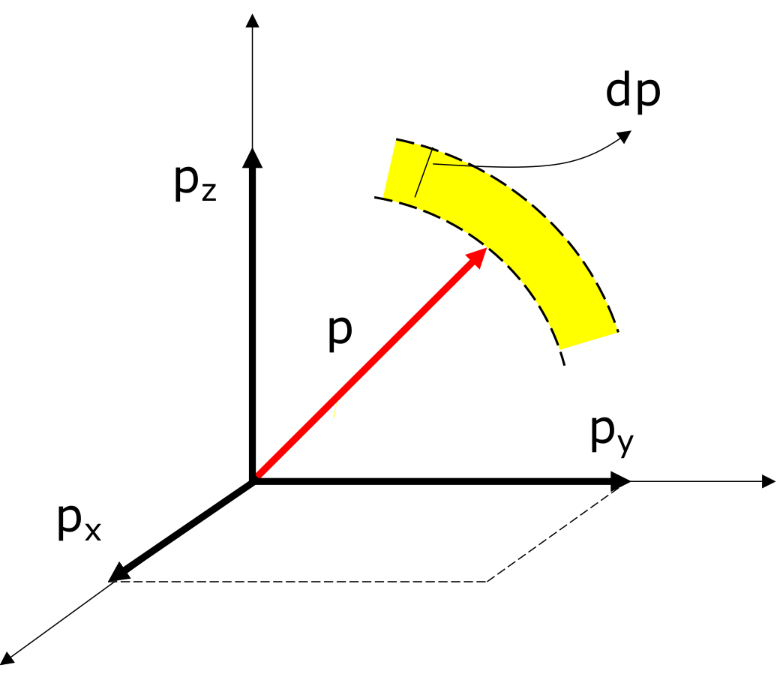
\includegraphics[width=0.3\textwidth]{immagini/volume-infinitesimo-sfera.png}
\caption{$\ud p_x \ud p_y \ud p_z$ è uguale al volume compreso tra due sfere concentriche di raggio $p$ e $p + \ud p$}
\label{fig:volume-infinitesimo-sfera}
\end{figure}

Sostituendo si trova la \emph{distribuzione di Fermi-Dirac}:
\begin{equation}\label{eq:fermi-dirac}
    N_p \ud p = \frac{8 \pi}{h^3} p^2 \ud p
\end{equation}
Si noti come essa \emph{non} dipenda da T. Per evidenziare l'emersione del comportamento quantistico oltre la soglia di Fermi, si faccia riferimento alla figura~\ref{fig:distribuzione-fermi}, in cui è rappresentato l'indice ci occupazione dei livelli energetici $\Pi(p)$ in funzione di $p$.

\begin{figure}
\centering
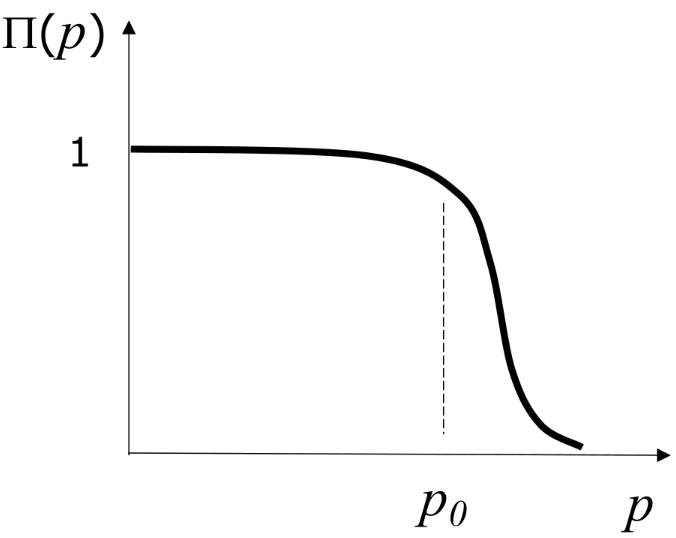
\includegraphics[width=0.3\textwidth]{immagini/distribuzione-fermi.png}
\caption{Indice di occupazione dei livelli energetici $\Pi(p)$ in funzione della quantità di moto $p$. $\Pi = 1$ corrisponde a un livello totalmente occupato.}
\label{fig:distribuzione-fermi}
\end{figure}

Integrando l'equazione~\eqref{eq:fermi-dirac} possiamo ottenere relazioni importanti in funzione del momento di Fermi. Si faccia attenzione al fatto che il massimo momento possibile è $p_0$, ovvero il momento di Fermi:
\[
N_e = \int_0^{p_0} \frac{8 \pi}{h^3} p^3 \ud p = \frac{8\pi}{3h^3} {p_0}^3
\]
dove $N_e$ rappresenta il numero di particelle per unità di volume. Sia $N_\textup{tot}$ il numero totale di particelle, $\langle m \rangle$ la massa media delle particelle, $M$ la massa totale e $V$ il volume. Si ha:
\[
N_e = \frac{N_\textup{tot}}{V} = \frac{M}{\langle m \rangle} \frac{1}{V} = \frac{\rho}{\mu_e H}
\]
dove è stata introdotta la densità $\rho$ e si è usata l'espressione~\eqref{eq:peso-molecolare-medio-definizione}.
Mettendo insieme le ultime due espressioni si ottiene:
\begin{equation}\label{eq:relazione-momento-fermi-densità}
    p_0 = \sqrt[3]{\dfrac{3h^3}{8\pi \mu_e H}} \rho^{1/3}
\end{equation}

Arrivati a questo punto, abbiamo tutti gli strumenti necessari per il calcolo della pressione. Come noto dalla meccanica statistica, conoscendo una distribuzione dei moduli di velocità, ipotizzando isotropia dello spazio, si può sempre trovare la pressione come:
\begin{equation}\label{eq:pressione-statistica}
    P = \frac{1}{3} m \int_0^\infty N(v) v^2 \ud v = \frac{1}{3m} \int_0^\infty N(p) p^2 \ud p
\end{equation}
e in generale bisogna distinguere tre casi:
\begin{description}
    \item[Gas perfetto] In questo caso la distribuzione di velocità da utilizzare è quella di Maxwell-Boltzmann. Integrando la~\eqref{eq:pressione-statistica} si ottiene la legge dei gas perfetti~\eqref{eq:gas-ideale}, in cui $\mu = \mu_e$.
    \item[Gas degenere non relativistico] La distribuzione di velocità è quella di Fermi Dirac. Si utilizza l'espressione classica per l'impulso, $p=mv$.
    \item[Gas degenere relativistico] La distribuzione di velocità è ancora quella di Fermi-Dirac, tuttavia si utilizza l'espressione relativistica per l'impulso, $p= \frac{m_e v}{\sqrt{1- (\frac{v}{c})^2}}$
\end{description}
Vediamo cosa si ottiene negli ultimi due casi.

\paragraph{Caso non relativistico}
In questo caso $p_0 \ll m_e c$ quindi possiamo scrivere $p=mv$ e integrare la~\eqref{eq:pressione-statistica} utilizzando la distribuzione di Fermi-Dirac~\eqref{eq:fermi-dirac}. Si ottiene:
\[
P = \dfrac{8\pi}{3h^3m} \int_0^{p_0} p^4 \ud p = \dfrac{8\pi}{3h^3m}\dfrac{{p_0}^5}{5}
\]
e sostituendo l'espressione per $p_0$ trovata precedentemente~\refeq{eq:relazione-momento-fermi-densità} otteniamo
\begin{equation}\label{eq:pressione-degenerazione-non-relativistica}
    P = k_1 \rho^{5/3}
\end{equation}
dove $k_1$ è una costante pari a:
\[
k_1 = 10^{13} {\mu_e}^{-5/3}
\]
Si noti come la pressione \emph{non} dipenda dalla temperatura. Questo fa sì che \emph{non} ci sia termoregolazione. Inoltre, la dipendenza dalla densità è maggiore rispetto che al gas perfetto (eq.~\eqref{eq:gas-ideale}).

\paragraph{Caso relativistico}
In questo caso si ha $p_0 \sim m_e c$ e bisogna utilizzare l'espressione relativistica dell'impulso:
\[
p= \dfrac{m_e v}{\sqrt{1- (\frac{v}{c})^2}}
\]
Sostituendo dentro~\eqref{eq:pressione-statistica} si ha:
\[
P = \dfrac{8\pi}{3mh^3} \int_0^{p_0} \dfrac{p^4 \ud p}{(1 + \dfrac{p^2}{m^2c^2})^{1/2}} = \dots = \dfrac{2\pi c}{3h^3}{p_0}^4
\]
dove si sono saltati i passaggi intermedi, riportati nel \emph{Cester}. Unendo l'ultima espressione con~\eqref{eq:relazione-momento-fermi-densità} si ottiene:
\begin{equation}\label{eq:pressione-degenerazione-relativistica}
    P = k_2 \rho^{4/3}
\end{equation}
con $k_2$ una costante pari a
\[
k_2 = 1.2 \cdot 10^{15} {\mu_e}^{-4/3}
\]
Nuovamente, non c'è dipendenza dalla temperatura e la dipendenza dalla densità è più forte che nel gas ideale~\eqref{eq:gas-ideale}.

\subsection{Richiami di Meccanica Statistica}
Ripassiamo quanto visto finora utilizzando le notazioni proposte nel corso istituzionale di Meccanica Statistica. Come sappiamo, per ciò che concerne l'occupazione energetica media è necessario distinguere tre tipi di particelle:
\begin{description}
\item[Classiche.] Esse seguono la distribuzione di Maxwell--Boltzmann. Consideriamo particelle di gas perfetto, pertanto esse saranno indistinguibili (cfr. paradosso di Gibbs). Lo spettro energetico è continuo.
\item[Fermioni.] Esse seguono la distribuzione di Fermi--Dirac, la quale tende a quella di Maxwell--Boltzmann nel limite classico. Lo spettro energetico è discreto con i vincoli del principio di esclusione di Pauli. 
\item[Bosoni.] Esse seguono la distribuzione di Bose--Einstein, la quale tende a quella di Maxwell--Boltzmann nel limite classico.
\end{description}

Nel caso delle particelle classiche, utilizzando il formalismo dell'ensamble grancanonico, si può calcolare la funzione di partizione grancanonica utilizzando il fatto che, per particelle indistinguibili, vale:
\[
Z(N) \simeq \frac{{Z_1}^N}{N!}
\]
con $Z(N)$ funzione di partizione canonica di $N$ particelle di gas perfetto e $Z_1$ funzione di partizione di una particella. Passando per il grande potenziale, è possibile trovare l'occupazione media per livello energetico. Si ottiene la distribuzione di Maxwell--Boltzmann:\
\begin{equation}
    \langle n_s  \rangle = e^{\beta(\mu - \epsilon_s)} 
\end{equation}

Nel caso di particelle quantistiche, invece, si calcola la funzione di partizione canonica sommando su tutti i possibili set di occupazione, utilizzando il vincolo $X=1$ per i fermioni (principio di Pauli) e $X=\infty$ per i bosoni, con $X$ il massimo valore possibile per un numero di occupazione. Sviluppando come sopra, si ottiene, nel primo caso, la distribuzione di Fermi--Dirac:
\begin{equation}
    \langle n_s \rangle = \dfrac{1}{e^{\beta(\epsilon_s - \mu)} + 1}
\end{equation}
Siamo interessati solamente a questa, poiché vogliamo studiare il comportamento degli elettroni, i quali, a causa del teorema Spin--Statistica, avendo spin semintero, si comportano collettivamente come fermioni.

Come noto, per temperature molto basse, $T \to 0$, la distribuzione di Fermi--Dirac assume la forma di una funzione a gradino di Heaviside, con numero di occupazione pari a $1$ per energie sotto l'energia di fermi ($\epsilon_F = \mu(T=0)$) e zero sopra. Si nota subito come la temperatura non possa più essere utilizzata per determinare l'energia del sistema, perché anche a temperature molto basse i fermioni si distribuiscono su livelli energetici sempre più alti a causa delle restrizioni del principio di esclusione. All'aumentare della temperatura la funzione di Fermi si arrotonda, poiché vi sarà energia termica a disposizione per permettere a qualche fermione di depositarsi su un livello energetico superiore alla soglia di Fermi. D'altra parte, per temperature molto alte, che corrispondono a una densità di particelle molto minore della concentrazione quantistica, la distribuzione tende a quella di Maxwell--Boltzmann.

Si ricorda, infatti, che un buon discriminante per determinare se una particella si comporta come classica o quantistica è la concentrazione quantistica. Essa si può trovare calcolando la funzione di partizione di una particella in una scatola cubica di potenziale con condizioni al contorno di annullamento, ed è pari a:
\begin{equation}\label{eq:concentrazione-quantistica}
    n_Q = \Bigl( \dfrac{m \kb T}{2 \pi {\hslash}^2}  \Bigr)^\frac{3}{2}, \qquad \lambda_\textup{th} = {n_Q}^{-\frac{1}{3}} 
\end{equation}
In particolare, se la densità $n$ di particelle è molto minore della concentrazione quantistica, $n \ll n_Q$, o equivalentemente se la distanza media tra due particelle è molto maggiore della lunghezza d'onda di De Broglie, $(V/N)^\frac{1}{3} \gg \lambda_\textup{th}$, le particelle possono essere trattate come classiche e la distribuzione di Maxwell--Boltmann sarà valida.

A questo punto ci si pone il problema di calcolare le pressioni di un gas perfetto e un gas di Fermi in condizione di forte degenerazione ($T \to 0$). Si vuole evidenziare un dettaglio: nonostante le temperature delle stelle siano relativamente elevate, esse possono essere considerate molto piccole rispetto alla \emph{temperatura di Fermi} della struttura, perciò è lecito trattare il gas di elettroni come se fosse a bassissima temperatura. 

Nel caso classico, come ovvio, si ottiene la legge dei gas perfetti. Nel caso quantistico si procede come segue. Prima di tutto, abbiamo necessità dell'espressione per la densità di stati, ovvero il numero di stati per unità di energia. Essa si può trovare risolvendo l'equazione di Schroedinger di una particella in una scatola di potenziale con condizioni di annullamento per trovare gli autovalori energetici. Siccome le autofunzioni dell'energia saranno proporzionali a dei seni, si imporrà che le pulsazioni debbano essere positive, da cui i numeri quantici dell'energia strettamente positivi. In particolare, si trova uno spettro energetico pari a:

\begin{equation}
    E_{n_x, \, n_y, \, n_z} = \dfrac{{\pi}^2 \hslash^2}{2mL^2} ({n_x}^2 + {n_y}^2 + {n_z}^2)
\end{equation}

Ora, per trovare la densità di stati ci metteremo nel k--spazio (lo spazio tridimensionale di versori $k_x$, $k_y$ e $k_z$), ricordando la condizione di quantizzazione del vettore d'onda derivante dall'annullamento della funzione d'onda sulle pareti della scatola, ovvero:

\begin{equation}
    E = \dfrac{k^2 \hslash^2}{2m}, \qquad \Vec{k} = \frac{\pi}{L} (n_x, n_y, n_z)
\end{equation}

Fissare un determinato valore di $k$ equivale a fissare l'impulso $p$, ovvero l'energia $E$, e ciò corrisponde a individuare un'ottante sferico nel k--spazio (a causa della condizione per cui $n_x, \, n_y, \, n_z > 0$). Dividendo il differenziale di ottante sferico $\frac{1}{8} 4\pi k^2 \ud k$ per il volume all'interno del quale è presente uno stato, equivalente al volume elementare $(\pi/L)^3$, si ottiene immediatamente la densità di stati, pari a:

\begin{equation}
    g(E) = \dfrac{\ud N}{\ud E} = \dfrac{g_s V }{4 {\pi}^2} \Bigl( \dfrac{2m}{\hslash^2} \Bigr)^\frac{3}{2} \sqrt{E}
\end{equation}
con $g_s$ la degenerazione di spin, $V$ il volume della scatola e $m$ la massa della particella.

Manca un ultimo ingrediente, ovvero il concetto di media termica. Ricordiamo che se $y(E)$ è una generica funzione dell'energia, conoscendo l'occupazione media per livello energetico $n(E)$, pari alla distribuzione di Maxwell--Boltzmann per particelle classiche o di Fermi--Dirac per fermioni, è possibile calcolare la media della funzione come:

\begin{equation}
    \langle y(E) \rangle = \dfrac{\sum_{E} n(E) y(E)}{\sum_E n(E)} = \frac{1}{N} \sum_{E} n(E) y(E) \to \frac{1}{N} \int_{0}^\infty \ud E \, n(E) \, g(E) \, y(E)
\end{equation}
dove, si faccia attenzione, la media è riferita alla singola particella, pertanto bisognerà moltiplicare per $N$ per ottenere la media riferita al sistema di particelle.

Per quanto detto precedentemente, gli elettroni in una stella possono essere trattati come un gas altamente degenere a causa dell'elevata temperatura di Fermi. Pertanto, possiamo calcolare in maniera molto semplice l'energia di Fermi supponendo di essere a $T=0$, condizione in cui la distribuzione di Fermi--Dirac è una distribuzione a scalino. Utilizzando la media termica per esprimere il numero medio di particelle abbiamo:

\[
N = \int_{0}^\infty \ud E \, g(E) \, n(E)
\]

Sostituendo tutti i valori ricordati sopra e sviluppando il conto, si può trovare l'energia di Fermi, corrispondente al potenziale chimico calcolato a $T=0$, trovando:

\begin{equation}\label{eq:energia-di-fermi}
    \mu(T=0) = \epsilon_F = \dfrac{\hslash^2}{2m} \Bigl( \dfrac{6 {\pi}^2 N}{g_s V} \Bigr) ^ \frac{2}{3}
 \end{equation}

 In maniera analoga si può calcolare l'energia interna usando nuovamente la definizione di media termica. Sviluppando i conti si trova:

 \begin{equation}\label{eq:energia-interna-di-fermi}
    U = \int_0^\infty \ud E \, g(E) \, E \, n(E) = \frac{3}{5} N \epsilon_F
 \end{equation}

 A questo punto si può procedere nel calcolo della pressione di un gas di Fermi in condizione di forte degenerazione utilizzando due risultati noti per il grande potenziale $\Phi$ del sistema grancanonico (si rimanda al Kennett per ulteriori dettagli):

 \[
    \Phi = PV, \qquad \Phi = \frac{2}{3} U
 \]
da cui è immediato trovare il valore della pressione di degenerazione, utilizzando le eq.~\eqref{eq:energia-di-fermi} e~\eqref{eq:energia-interna-di-fermi}. Si ottiene:

\begin{equation}\label{eq:pressione-degenerazione-kennett}
    P = \frac{2}{3} \frac{U}{V} = \frac{2}{5} \frac{N}{V} \epsilon_F
\end{equation}

Infine, riconosciamo che la densità del gas è proporzionale al numero di particelle, $\rho \propto N$, e siccome nell'espressione precedente abbiamo un termine $\propto N$ derivante dall'espressione dell'energia~\eqref{eq:energia-interna-di-fermi} e un termine $\propto N^\frac{2}{3}$ derivante dall'energia di Fermi~\eqref{eq:energia-di-fermi}, troviamo che la pressione di degenerazione deve essere proporzionale a $N^\frac{5}{3} \propto \rho^\frac{5}{3}$, da cui si ottiene la formula dell'equazione di stato:

\[
  P = k_1 \rho^\frac{5}{3}  
\]

Tralasciando il caso non relativistico, rivediamo in breve tutti i termini dell'equazione di stato.

\subsection{L'equazione in breve}
L'equazione di stato negli interni stellari~\eqref{eq:equazione-stato} ha tre contributi principali. Analizziamoli celermente.

\paragraph{Pressione di radiazione}
Il termine:
\[
P = \dfrac{aT^4}{3}
\]
rappresenta il contributo della pressione di radiazione per un corpo nero, secondo la eq.~\eqref{eq:pressione-radiazione} ottenuta integrando la distribuzione di Planck~\refeq{eq:corpo-nero}. È il contributo dei fotoni che compongono il gas stellare, i quali hanno un impulso e dunque esercitano una pressione.

\paragraph{Pressione degli ioni}
Il termine:
\[
\dfrac{k \rho T}{\mu_i H}
\]
è il contributo degli ioni nel materiale stellare, che pensiamo come a un plasma. Questi sono sempre approssimati come a un gas perfetto, infatti seguono la legge~\eqref{eq:gas-ideale}.

\paragraph{Pressione degli elettroni}
Il contributo:
\[
\begin{cases} 
    \dfrac{k \rho T}{\mu_e H} \\ 
    k_1 \rho^{5/3} \\ 
    k_2 \rho^{4/3}
    \end{cases}
\]
dipende dalla degenerazione del gas per ciò che concerne il contributo elettronico. Se il gas di elettroni è \emph{non} degenere, ovvero è un gas perfetto, segue la legge~\eqref{eq:gas-ideale}, dove $\mu = \mu_e$. Nel caso \emph{degenere} si distinguono due situazioni: la prima in cui si trattano le particelle come \emph{non} relativistiche, con un contributo alla pressione pari a $k_1 \rho^{5/3}$, e un secondo in cui si trattano le particelle come \emph{relativistiche}, con un contributo alla pressione pari a $k_2 \rho^{4/3}$.

\subsection{Contributo dominante}
Per descrivere lo stato della materia negli interni stellari, è utile utilizzare il \emph{diagramma} $\log \rho$ -- $\log T$. In pratica, note la densità e la temperatura di un certo strato di stella, questo piano permette di sapere quale componente di pressione prevale. Infatti, eguagliando tra loro diversi contributi di pressione, si ottengono delle rette che suddividono il piano in regioni in cui domina l'uno o l'altro contributo. Analizziamo i domini di demarcazioni per casi. Nella figura~\ref{fig:diagramma-logrho-logt} sono mostrati tutti i casi. Essa è riferita al nucleo stellare, in cui le temperature sono elevatissime, in superficie le temperature sono più basse.

\begin{figure}
\centering
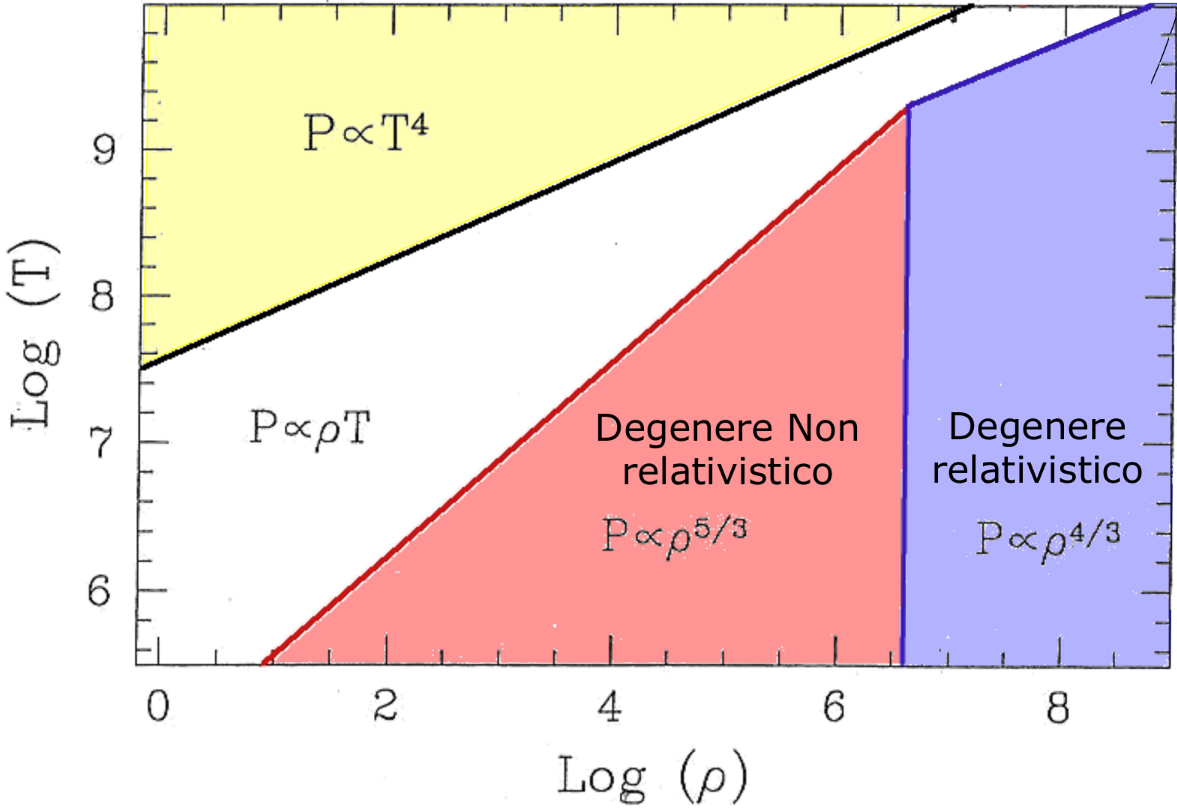
\includegraphics[width=0.5\textwidth]{immagini/piano-log-log.png}
\caption{Diagramma $\log \rho$ -- $\log T$. In giallo domina la pressione di radiazione, in bianco il gas non degenere (gas perfetto), in rosso il gas degenere non relativistico e in blu il gas degenere relativistico.}
\label{fig:diagramma-logrho-logt}
\end{figure}

\paragraph{Pressione di radiazione -- Pressione del gas perfetto}
Imponiamo $P_\textup{rad} = P_\textup{gas}$, uguagliando dunque l'eq.~\eqref{eq:pressione-radiazione} con l'eq.~\eqref{eq:gas-ideale}. In pratica sto considerando insieme il contributo degli ioni e degli elettroni, utilizzando $1/ \mu_i + 1 / \mu_e = 1 / \mu$
\[
\frac{1}{3} a T^4 = \frac{\kb \rho T}{\mu H}
\]
sviluppando si trova:
\[
T^3 = \dfrac{3\kb}{a\mu H} \rho
\]
da cui, passando ai logaritmi:
\[
\log T^3 = \log \rho + c
\]
e infine si può ricavare:
\begin{equation}\label{prad-pgas}
    \log T = \frac{1}{3} \log \rho + 7.57
\end{equation}
La regione in giallo del diagramma~\ref{fig:diagramma-logrho-logt} è quella in cui la pressione di radiazione domina su quella del gas perfetto, ovvero $P_\textup{rad} > P_\textup{gas}$

\paragraph{Pressione del gas degenere -- Pressione del gas perfetto}
Per sapere quando la pressione del gas degenere di elettroni prevale su quella di gas perfetto, uguagliamo la~\eqref{eq:gas-ideale} con la~\eqref{eq:pressione-degenerazione-non-relativistica}. Siccome la condizione di degenerazione riguarda solamente il contributo elettronico, nella parte del gas perfetto considero solo gli elettroni, per cui $\mu = \mu_e$:
\[
\frac{\kb \rho T}{\mu_e H} = k_1 \rho^{5/3}
\]
da cui si ottiene:
\[
T = \frac{k_1}{\kb} \rho^{2/3} \mu_e H
\]
e, passando ai logarirtmi:
\begin{equation}\label{eq:pgas-pdeg}
    \log T = \frac{2}{3} \log \rho + 4.88
\end{equation}
La regione in rosso del diagramma~\ref{fig:diagramma-logrho-logt} è quella in cui la pressione del gas degenere è maggiore della pressione del gas non degenere.

\paragraph{Pressione del gas degenere relativistico -- Pressione del gas degenere non relativistico}
Per sapere quando la pressione del gas degenere relativistico prevale su quella del gas degenere \emph{non} relativistico, uguagliamo la~\eqref{eq:pressione-degenerazione-non-relativistica} con la~\eqref{eq:pressione-degenerazione-relativistica}:
\[
k_1 \rho^{5/3} = P = k_2 \rho^{4/3}
\]
si trova:
\[
\rho^{1/3} = \frac{k_2}{k_1}
\]
da cui, passando ai logaritmi:
\begin{equation}\label{eq:pdegrel-pdegnonrel}
    \log \rho = 3 \log \frac{k_2}{k_1} = 6.6
\end{equation}
La pressione in blu del diagramma~\ref{fig:diagramma-logrho-logt} è quella in cui la pressione del gas degenere relativistico è maggiore di quella del gas degenere non relativistico.

\paragraph{Pressione del gas perfetto -- Pressione del gas degenere relativistico}
Analogamente a quanto fatto nel caso \emph{non} relativistico, ci sarà una regione del diagramma (per $\log \rho > 6.6$) in cui il gas può passare da \emph{non degenere} a \emph{degenere relativistico}. Per trovarla uguagliamo la~\eqref{eq:gas-ideale} con la~\eqref{eq:pressione-degenerazione-relativistica}:
\[
\frac{\kb \rho T}{\mu H} = k_2 \rho^{4/3}
\]
si trova:
\[
T = \frac{k_2 \mu_e H}{\kb} \rho^{1/3}
\]
e passando ai logaritmi:
\begin{equation}\label{eq:pgas-pdegrel}
    \log T = \frac{1}{3} \log \rho + 7.07
\end{equation}

\paragraph{Conclusioni}
La pressione di radiazione, siccome $p_\textup{rad} \propto T^4$, domina ad alte temperature. La pressione del gas degenere diventa dominante ad alte densità perché per avere degenerazione devo avere gli elettroni estremamente impacchettati nello spazio delle fasi, e ciò corrisponde ad elevate densità. Nei casi intermedi è sufficiente riferirsi al grafico~\ref{fig:diagramma-logrho-logt} per capire in quale situazione si è.

Riprenderemo questo utile diagramma successivamente, parlando di evoluzione stellare. Per ora sottolineamo solamente che le reazioni termonucleari sono attive solo se il gas si trova in condizioni di non degenerazione (gas perfetto).